\section{The Pole and Barn Paradox}

\makelabheader %(Space for student name, etc., defined in master.tex)

\instructornote{%
By Matt Trawick, added to 131 in 2019.  Time: 35 minutes

This lab has been used in Modern for many years before 2019.  It assumes students are familiar with the ideas of length contraction and Lorentz transforms.  It doesn't give a lot of introduction to the Mathematica simulation, so it probably kind of assumes they've seen that before in previous labs too.  Good preparation for this would be the lab ``Galilean Transformations and Lorentz Transformations.''

Otherwise, there is no specific introduction necessary for this lab; it is self-contained, in the sense that you don't need to explain this specific paradox before they start.

Often, a student will ask the question, ``What if the front end of the pole doesn't go through the right-hand barn door, but stops instantly.  Then don't Bob and Anna disagree where the pole stops?''  The resolution to this is that information that the front end has stopped can only travel to the back end at speed c, and by the time it gets there both Anna and Bob agree that the back end of the pole is inside the barn.  This is illustrated by the file pole\_and\_barn\_complete.nb.  I usually don't deal with that issue on the day of the lab, but assign a problem about it for homework afterwards, and discuss it the following day.
}

\medskip
\textbf{Apparatus:}
\begin{itemize}[nosep]
\item \textit{Mathematica}, with notebook file \filename{pole\_and\_barn.nb}
\end{itemize}

\medskip

Anna has recently taken up pole vaulting, and owns a 10-meter-long pole (its proper length).  Bob has taken up farming, and owns an 8-meter-long barn (also its proper length) with a door on each end.  Anna holds her pole and runs at $v=+0.8 c$ towards one of the open barn doors.  
%The right end of the pole enters the barn at $x = 0$, at some time $t < 0$, and the left end of the pole enters the barn at $x = 0$ and $t = 0$.
\begin{center}
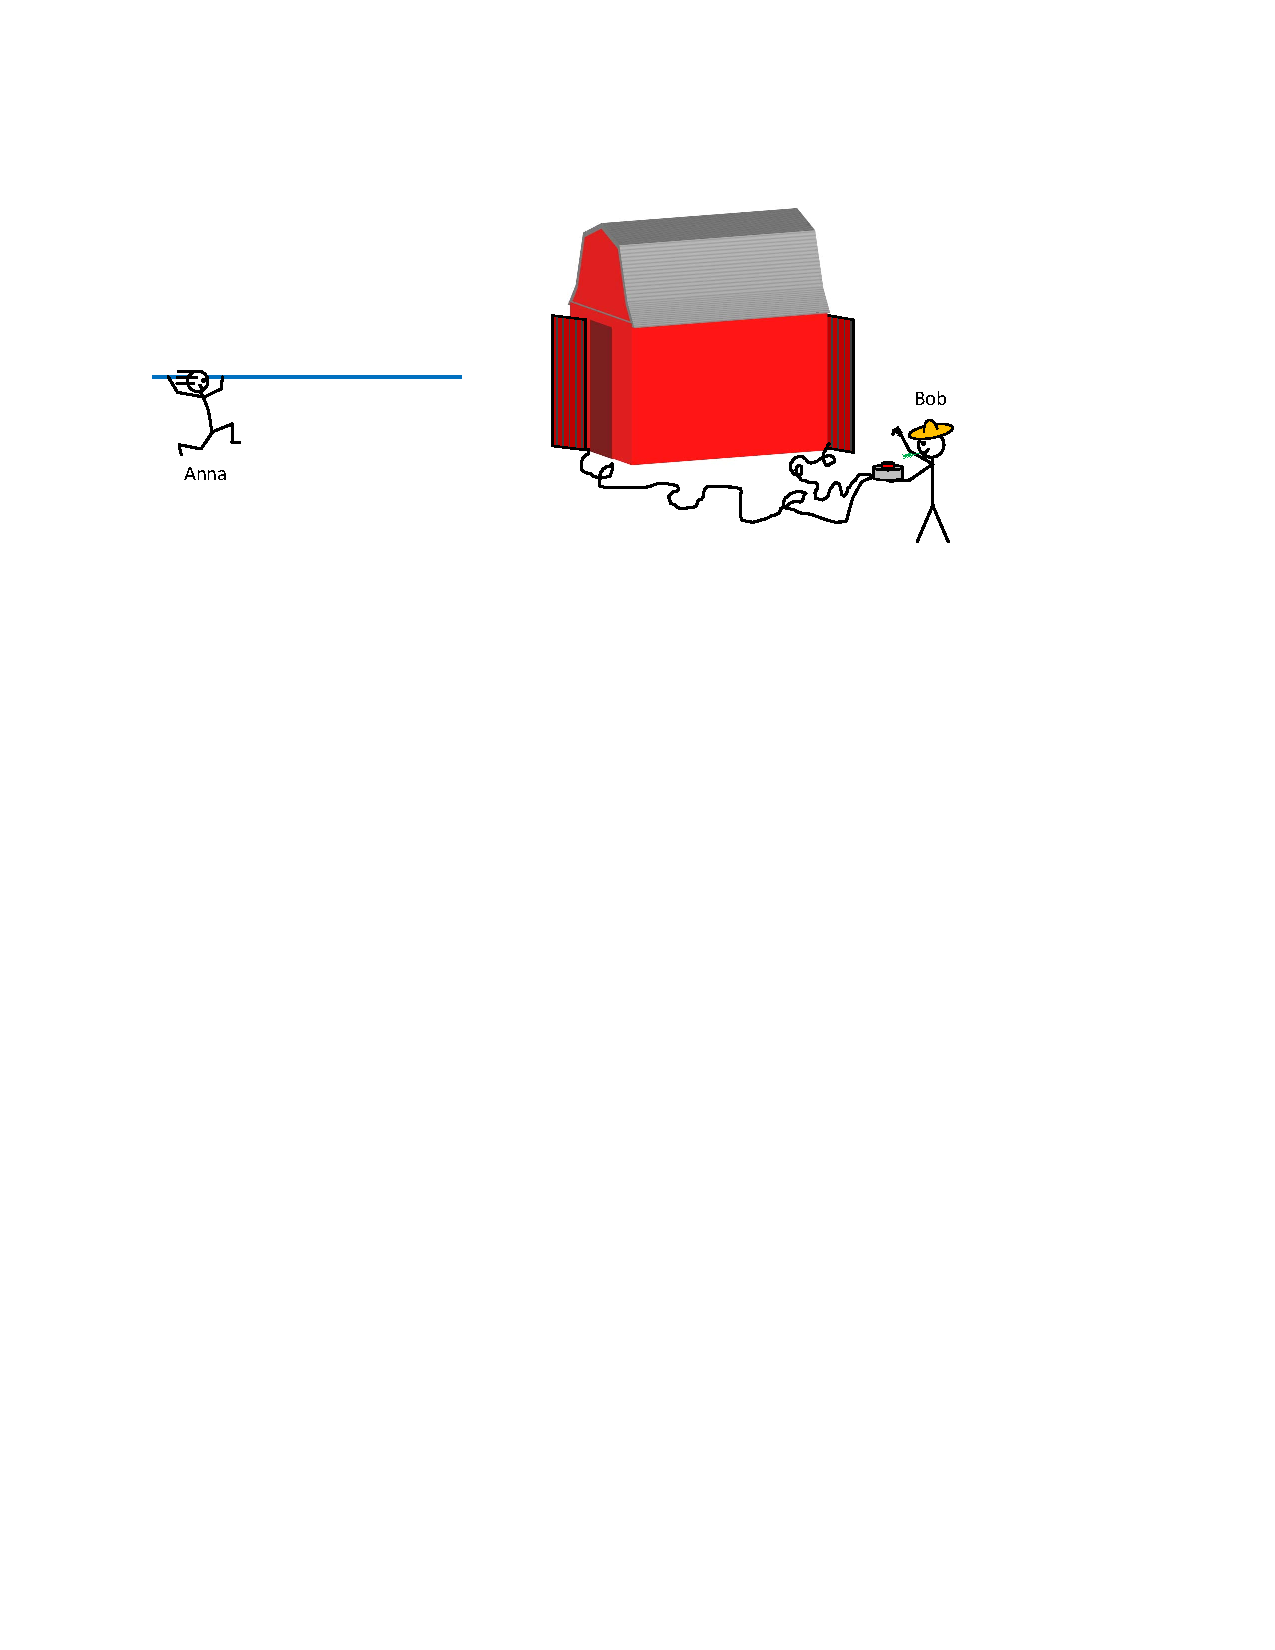
\includegraphics{pole_and_barn/pole_and_barn_drawing.pdf}
\index{color page}
\end{center}
Here's what happens, according to farmer Bob, standing beside the barn:
\begin{itemize}[nosep,topsep=-\parskip]
\item The pole is length-contracted so that it is shorter than the barn.
\item When the pole is centered inside the barn, Bob pushes a button so that both doors shut very quickly with the pole entirely inside the barn.
\item Bob says, ``Ah-ha! I've closed Anna's pole inside the barn!''
\end{itemize}

\medskip
But here's what happens according to Anna:
\begin{itemize}[nosep,topsep=-\parskip]
\item Her pole is 10 meters long.
\item The barn is length-contracted to less than 8 meters long.
\item Anna says, ``My pole couldn't possibly have been closed inside the barn.  It wouldn't even fit inside!''
\end{itemize}

\medskip
This seems like a paradox, since both observers have to agree on any tangible outcome of an experiment!

\medskip

%\textbf{Activity 1: Understanding the paradox}
% if adding a second activity, change ``wide, nosep'' below to ``labparts''

\begin{enumerate}[wide, nosep]
\item Open the file \filename{pole\_and\_barn.nb} in Mathematica. If you get a pop-up error message, you may need to click \button{Enable Dynamic Content}. Type \button{Ctrl-A} to select all lines, and hit \button{Shift-Enter} to execute them. The graph you see represents a ``spacetime diagram'' (or ``Minkowski diagram'') of this set of events, with $x$ on the horizontal axis and $t$ on the vertical axis. If the units on the horizontal axis are in meters, and the diagonal dotted lines represent objects traveling from the origin at the speed of light, what are the units of the vertical (time) axis?
\answerspace{0.3in}

\item With the velocity slider set to $v = 0$ (the default), the diagram is in the reference frame of farmer Bob. The red lines represent the positions in time, or \textit{worldlines}, of the two barn doors, and the purple lines represent the worldlines of the two ends of Anna's pole. Based on this diagram, what is the approximate length of Anna's pole according to Bob?  \label{part_approx_pole_length}
\answerspace{0.3in}

\item Verify your answer in part~\ref{part_approx_pole_length} by doing a calculation to determine the precise length contraction of the pole according to Bob.
\answerspace{0.6in}

\item Now, move the slider so that you view these events from Anna's reference frame.
From the graph, how long is the barn according to Anna? \label{part_approx_barn_length}
\answerspace{0.3in}

\item Verify your reading of the graph in part~\ref{part_approx_barn_length} by calculating the precise length of the barn in Anna's reference frame.
\answerspace{0.6in}

\item Now move the slider back to Bob's reference frame. According to Bob, at what time is the pole exactly centered inside the barn?
\answerspace{0.6in}

\item There are two red dots in the graph at random locations. Edit the Mathematica file in the line that looks like
$$\verb!ListPlot[{lorentz[-3,3,v],lorentz[-3,4.5,v]},PlotStyle ->{PointSize[Large],Red}]!$$
to change the coordinates of those dots so that they mark the space and time coordinates of the closing of the two barn doors in Bob's reference frame. What are those exact coordinates?
\answerspace{0.8in}

\item The table below lists six distinct events.  Write the order (1 through 6) in which these events occur in Bob's reference frame, indicating any events that happen simultaneously.  

\begin{center}
{\renewcommand{\arraystretch}{1.8}
\begin{tabular}{|l|C{1.0in}|C{1.0in}|} \hline 
\textbf{Event Description} & \textbf{Bob's Order} & \textbf{Anna's Order} \\ 
\hhline{|=|=|=|}
Front of Anna's pole at left barn door & & \\ \hline 
Back of Anna's pole at left barn door & & \\ \hline 
Left barn door closes & & \\ \hline 
Right barn door closes & & \\ \hline 
Front of Anna's pole crashes through right barn door & & \\ \hline 
Back of Anna's pole at right barn door & & \\ \hline 
\end{tabular} }
\end{center}

\item Now move the slider back to Anna's reference frame. In the table above, write the order (1 through 6) in which the events occur in Anna's reference frame.  

\item So, was the pole ever closed inside the barn or not? Who has the ``correct'' view---Anna? Bob? Neither? Both?  Don't all observers need to agree on the outcome of an experiment?  
\medskip

Write an explanation that resolves the apparent paradox of the pole and the barn. 
(Hint: Your explanation will surely be based on in the idea that observers in different reference frames can measure events occurring different times, and that events that are simultaneous in one frame may not be simultaneous in another.  
\textbf{But to fully explain the paradox, you will need to clearly define \textit{exactly} what it means for an object to be ``closed inside'' a barn with two doors.})
\answerspace{1.5in}

\end{enumerate}

%\textbf{Activity 2: But what if Anna stops?}

%\begin{enumerate}[labparts]
